%%%%%%%%%%%%%%%%%%%%%%%%%%%%%%%%%%%%%%%%%
% Jacobs Landscape Poster
% LaTeX Template
% Version 1.0 (29/03/13)
%
% Created by:
% Computational Physics and Biophysics Group, Jacobs University
% https://teamwork.jacobs-university.de:8443/confluence/display/CoPandBiG/LaTeX+Poster
% 
% Further modified by:
% Nathaniel Johnston (nathaniel@njohnston.ca)
%
% This template has been downloaded from:
% http://www.LaTeXTemplates.com
%
% License:
% CC BY-NC-SA 3.0 (http://creativecommons.org/licenses/by-nc-sa/3.0/)
%
%%%%%%%%%%%%%%%%%%%%%%%%%%%%%%%%%%%%%%%%%

% Taken from https://www.overleaf.com/latex/templates/landscape-beamer-poster-template/vjpmsxxdvtqk

%----------------------------------------------------------------------------------------
%	PACKAGES AND OTHER DOCUMENT CONFIGURATIONS
%----------------------------------------------------------------------------------------

\documentclass[final]{beamer}

\usepackage[scale=1.24]{beamerposter} % Use the beamerposter package for laying out the poster

\usetheme{confposter} % Use the confposter theme supplied with this template

\setbeamercolor{block title}{fg=ngreen,bg=white} % Colors of the block titles
\setbeamercolor{block body}{fg=black,bg=white} % Colors of the body of blocks
\setbeamercolor{block alerted title}{fg=white,bg=dblue!70} % Colors of the highlighted block titles
\setbeamercolor{block alerted body}{fg=black,bg=dblue!10} % Colors of the body of highlighted blocks
% Many more colors are available for use in beamerthemeconfposter.sty

%-----------------------------------------------------------
% Define the column widths and overall poster size
% To set effective sepwid, onecolwid and twocolwid values, first choose how many columns you want and how much separation you want between columns
% In this template, the separation width chosen is 0.024 of the paper width and a 4-column layout
% onecolwid should therefore be (1-(# of columns+1)*sepwid)/# of columns e.g. (1-(4+1)*0.024)/4 = 0.22
% Set twocolwid to be (2*onecolwid)+sepwid = 0.464
% Set threecolwid to be (3*onecolwid)+2*sepwid = 0.708

\newlength{\sepwid}
\newlength{\onecolwid}
\newlength{\twocolwid}
\newlength{\threecolwid}
\setlength{\paperwidth}{48in} % A0 width: 46.8in
\setlength{\paperheight}{36in} % A0 height: 33.1in
\setlength{\sepwid}{0.024\paperwidth} % Separation width (white space) between columns
\setlength{\onecolwid}{0.22\paperwidth} % Width of one column
\setlength{\twocolwid}{0.464\paperwidth} % Width of two columns
\setlength{\threecolwid}{0.708\paperwidth} % Width of three columns
\setlength{\topmargin}{-0.5in} % Reduce the top margin size
%-----------------------------------------------------------

\usepackage{graphicx}  % Required for including images
\graphicspath{{figures/}{logos/}}

\usepackage{booktabs} % Top and bottom rules for tables

%----------------------------------------------------------------------------------------
%	TITLE SECTION 
%----------------------------------------------------------------------------------------

\title{Cracking Neural Network Hashes with Adversarial Examples}

\author{Conrad Christensen, Da Ying}

\institute{Computer Science, New York University} % Institution(s)

%----------------------------------------------------------------------------------------

\begin{document}

\addtobeamertemplate{block end}{}{\vspace*{2ex}} % White space under blocks
\addtobeamertemplate{block alerted end}{}{\vspace*{2ex}} % White space under highlighted (alert) blocks

\setlength{\belowcaptionskip}{2ex} % White space under figures
\setlength\belowdisplayshortskip{2ex} % White space under equations

\begin{frame}[t] % The whole poster is enclosed in one beamer frame

\begin{columns}[t] % The whole poster consists of three major columns, the second of which is split into two columns twice - the [t] option aligns each column's content to the top

\begin{column}{\sepwid}\end{column} % Empty spacer column

\begin{column}{\onecolwid} % The first column

%----------------------------------------------------------------------------------------
%	OBJECTIVES
%----------------------------------------------------------------------------------------

\begin{alertblock}{Objective}
    In this project we seek to show that hash functions, implemented as neural
    networks, are susceptible to gradient-based attacks that can generate 
    collisions.
\end{alertblock}

%----------------------------------------------------------------------------------------
%	INTRODUCTION
%----------------------------------------------------------------------------------------

\begin{block}{Introduction}
    A cryptographic hash function is a function used to
    reduce documents into a fixed size hash.
    These functions
    must be \emph{one-way}, hence given hash of a document, it is infeasible to find a document
    that produces the same hash \cite{crypoHash}.  

    The problem of finding good cryptographic hash functions using neural networks has
    been proposed in multiple papers \cite{hash1, hash2}. We believe these
    functions fundamentally do not satisfy the one-way requirement for
    cryptographic hashes as they expose important information through their
    differentiability.
\end{block}

%------------------------------------------------

\begin{figure}
    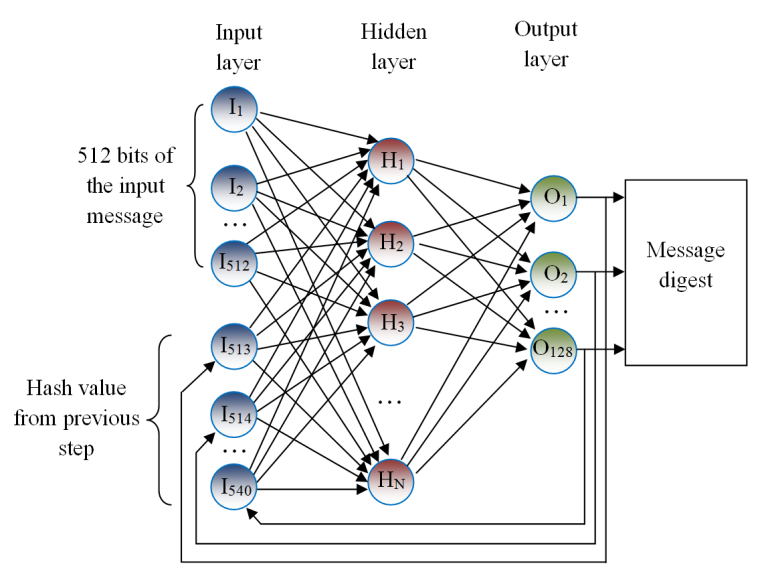
\includegraphics[width=0.8\linewidth]{hash_nn_architecture}
    \caption{Hash function algorithm presented in \cite{hash1}}
    \label{fig:hashNN}
\end{figure}

\begin{figure}
    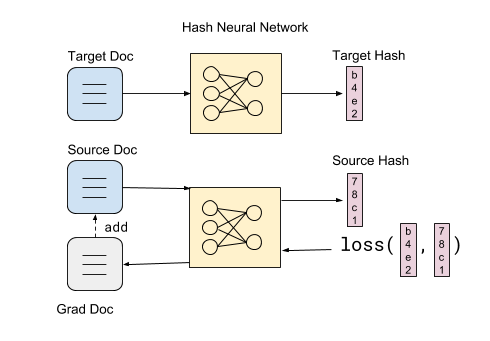
\includegraphics[width=0.8\linewidth]{model_diagram}
        \caption{Collision attack overview} 
        \label{fig:model}
\end{figure}


%----------------------------------------------------------------------------------------

\end{column} % End of the first column

\begin{column}{\sepwid}\end{column} % Empty spacer column

\begin{column}{\twocolwid} % Begin a column which is two columns wide (column 2)

\begin{columns}[t,totalwidth=\twocolwid] % Split up the two columns wide column

\begin{column}{\onecolwid}\vspace{-.6in} % The first column within column 2 (column 2.1)

%----------------------------------------------------------------------------------------
%	MATERIALS
%----------------------------------------------------------------------------------------

\begin{block}{Neural Hash Function}
The model that we will be attacking here, for the purpose of demonstrating
issues with neural network cryptographic hash functions, is that described
in \cite{hash1}.  Here a two-layer recurrent neural network (RNN)
reads 512 bit blocks, combines them with the output of the previous block,
and produces 128 bit output (see Figure \ref{fig:hashNN}).

\begin{itemize}
    \item The RNN has two linear layers
    \item Sigmoid activation at each layer
    \item Input layer takes 640 bits (512 bit block and 128 bits from last 
        block) and produce 128 bit output
    \item Weights are randomly initialized once (so function is deterministic)
\end{itemize}

\end{block}

%----------------------------------------------------------------------------------------

\end{column} % End of column 2.1

\begin{column}{\onecolwid}\vspace{-.6in} % The second column within column 2 (column 2.2)

%----------------------------------------------------------------------------------------
%	METHODS
%----------------------------------------------------------------------------------------

\begin{block}{Results}

We evaluate the performance of our model, the success rate to generate pseudo-collisions and the average time it takes. The first factor we take into consideration is the size of source file. Figures \ref{fig:docsize} shows the model achieves 100\% success rate when the size of source doc reaches 512 bytes. When size of source document is too small, the model lacks of information and value to change to reach the target hash. It also shows the larger the source doc, the longer it takes to generate the collisions. When there is no restriction on choosing source documents, a documents with random 512 bytes gives the best performance.

\end{block}

%----------------------------------------------------------------------------------------

\end{column} % End of column 2.2

\end{columns} % End of the split of column 2 - any content after this will now take up 2 columns width

%----------------------------------------------------------------------------------------
%	IMPORTANT RESULT
%----------------------------------------------------------------------------------------

\begin{alertblock}{Important Result}
    Collisions we found were \emph{pseudo-collisions}. This means that while the
    source document did produce the same hash as the target document, the souce
    document's bits deviated from the valid values of 0 and 1.
\end{alertblock} 

%----------------------------------------------------------------------------------------

\begin{columns}[t,totalwidth=\twocolwid] % Split up the two columns wide column again

\begin{column}{\onecolwid} % The first column within column 2 (column 2.1)

%----------------------------------------------------------------------------------------
%	MATHEMATICAL SECTION
%----------------------------------------------------------------------------------------

\begin{block}{Our Model}
Our attack exploits the fact that the RNN itself is differentiable, so with a loss
function that pushes one hash value to another, we can generate colliding
hash values.
This method can be realized through the following steps (see Figure \ref{fig:model}):
\begin{enumerate}
    \item Choose a target hash value, and source document
    \item Hash source document to get source hash
    \item Calculate MSE loss of source hash with target hash
    \item Add extra loss term to penalize source document bits that deviate from 0 or 1
    \item Back-propagate loss to get gradient of loss w.r.t. source document
    \item Add gradient to source document to get new source document
    \item Repeat until source hash equals target hash
\end{enumerate}
\end{block}

%----------------------------------------------------------------------------------------

\end{column} % End of column 2.1

\begin{column}{\onecolwid} % The second column within column 2 (column 2.2)

%----------------------------------------------------------------------------------------
%	RESULTS
%----------------------------------------------------------------------------------------

\begin{block}{Results cont.}

\begin{figure}
    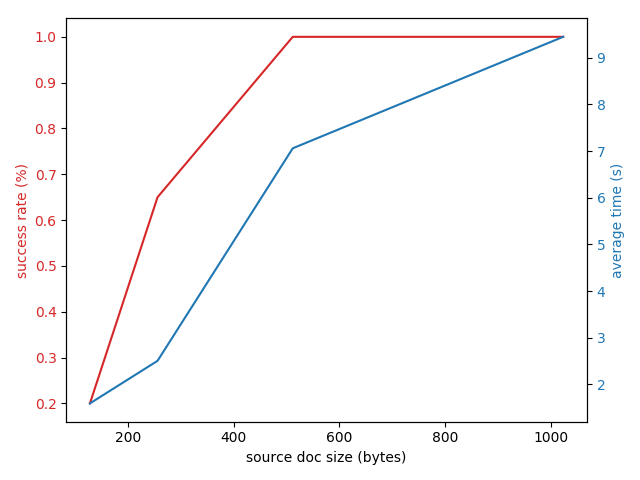
\includegraphics[width=0.8\linewidth]{source_doc_size}
    \caption{Performance for different sizes of source docs}
    \label{fig:docsize}
\end{figure}

Figure \ref{fig:lrate} shows when learning rate is less than 1.0 or larger than 1.5, the model will have the risk of getting stuck in the local minimums, or failure to converge in time. The difference on distribution of the final source documents value is minimal with different regularization coefficients in Figure \ref{fig:datadist}.

\end{block}

%----------------------------------------------------------------------------------------

\end{column} % End of column 2.2

\end{columns} % End of the split of column 2

\end{column} % End of the second column

\begin{column}{\sepwid}\end{column} % Empty spacer column

\begin{column}{\onecolwid} % The third column


\begin{figure}
    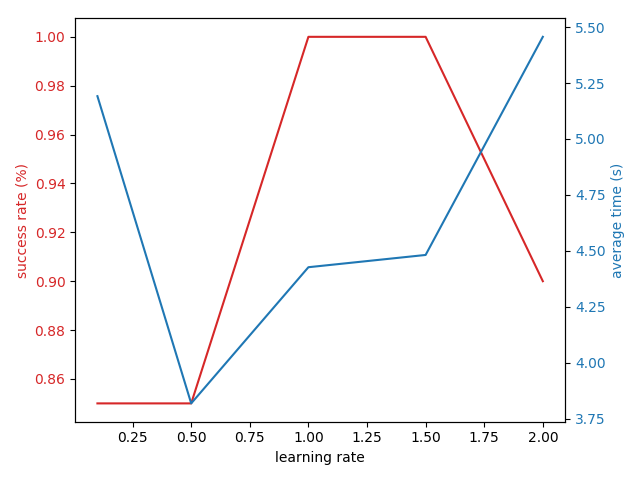
\includegraphics[width=0.8\linewidth]{learning_rate}
        \caption{Performance for different learning rates} 
        \label{fig:lrate}
\end{figure}

\begin{figure}
    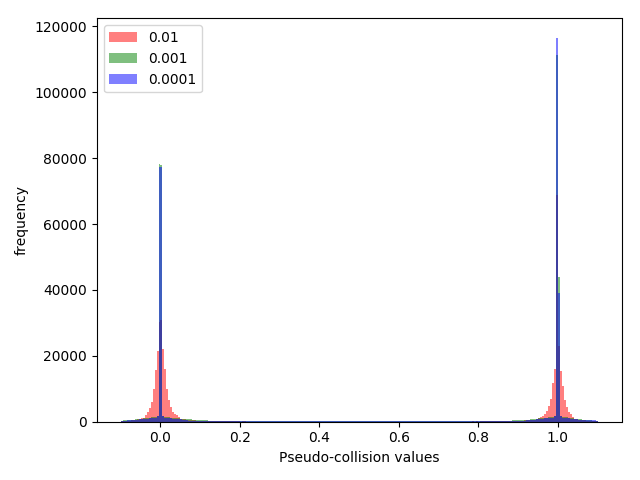
\includegraphics[width=0.8\linewidth]{data_distribution}
        \caption{Pseudo-collisions value distribution for different regularization coefficient} 
        \label{fig:datadist}
\end{figure}


%----------------------------------------------------------------------------------------
%	CONCLUSION
%----------------------------------------------------------------------------------------

\begin{block}{Conclusion}
    We have shown that a neural network hash function does suffer from a strong
    weakness due to its differentiability. We have shown that it is possible
    to generate pseudo-collisions, and we believe, with a little more work,
    real collisions.
\end{block}

%----------------------------------------------------------------------------------------
%	ADDITIONAL INFORMATION
%----------------------------------------------------------------------------------------

%\begin{block}{Additional Information}

%Maecenas ultricies feugiat velit non mattis. Fusce tempus arcu id ligula varius dictum. 
%\begin{itemize}
%\item Curabitur pellentesque dignissim
%\item Eu facilisis est tempus quis
%\item Duis porta consequat lorem
%\end{itemize}

%\end{block}

%----------------------------------------------------------------------------------------
%	REFERENCES
%----------------------------------------------------------------------------------------

\begin{block}{References}
    \tiny{See paper for full list of citations}
%\nocite{*} % Insert publications even if they are not cited in the poster
\small{\bibliographystyle{unsrt}
\bibliography{ref}\vspace{0.75in}}

\end{block}

%----------------------------------------------------------------------------------------
%	ACKNOWLEDGEMENTS
%----------------------------------------------------------------------------------------

%\setbeamercolor{block title}{fg=red,bg=white} % Change the block title color

%\begin{block}{Acknowledgements}

%\small{\rmfamily{Nam mollis tristique neque eu luctus. Suspendisse rutrum congue nisi sed convallis. Aenean id neque dolor. Pellentesque habitant morbi tristique senectus et netus et malesuada fames ac turpis egestas.}} \\

%\end{block}

%%----------------------------------------------------------------------------------------
%%	CONTACT INFORMATION
%%----------------------------------------------------------------------------------------

%\setbeamercolor{block alerted title}{fg=black,bg=norange} % Change the alert block title colors
%\setbeamercolor{block alerted body}{fg=black,bg=white} % Change the alert block body colors

%\begin{alertblock}{Contact Information}

%\begin{itemize}
%\item Web: \href{http://www.university.edu/smithlab}{http://www.university.edu/smithlab}
%\item Email: \href{mailto:john@smith.com}{john@smith.com}
%\item Phone: +1 (000) 111 1111
%\end{itemize}

%\end{alertblock}

\begin{center}
%\begin{tabular}{ccc}
%
\includegraphics[width=0.8\linewidth]{nyu_short} & \hfill & 
\includegraphics[width=0.4\linewidth]{nyu_data_science.png}
%
\includegraphics[width=0.8\linewidth]{nyu_data_science.png}\\

\includegraphics[width=0.8\linewidth]{nyu_long.png}
%\end{tabular}
\end{center}

%----------------------------------------------------------------------------------------

\end{column} % End of the third column

\end{columns} % End of all the columns in the poster

\end{frame} % End of the enclosing frame

\end{document}
